\textbf{\subsection{Расчет оконечного каскада}}
\vspace{1em}

Оконечный каскад представляет собой элемент усиления мощности схемы УМ, выполненный на транзисторах n-p-n (VT4) и p-n-p (VT5), представляющих собой двухтактный каскад. Для достижения усиления мощности транзисторы VT4 и VT5 работают в режиме B, за счет которого достигается большой КПД, т.к. ток в выходной цепи протекает только в течение половины периода. За счет включения в выходном каскаде двух транзисторов: n-p-n и p-n-p, достигается прохождение в выходной цепи сигнала в течение всего периода, что способствует работе каскада в непрерывном режиме. 

\begin{figure}[!htbp]
    \center{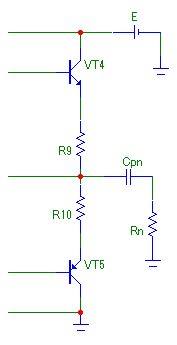
\includegraphics[width=0.23\linewidth]{picture_ok}}
    \caption{Схема оконечного каскада}
    \label{figure:p2_3}
  \end{figure}

Резисторы R9 и R10, включенные в цепи эмиттеров транзисторов, представляют местную обратную связь. \par
Усиление по мощности достигается за счет усиления по току.


\subsubsection{Определяем амплитуду напряжения и тока на нагрузке}

\begin{equation}
\label{eq:equation2_1}
 U_{\text{нм}} = \sqrt{2 P_{\text{н}} R_{\text{н}}}
\end{equation}

\begin{equation*}
 U_{\text{нм}} = \sqrt{ 2 \cdot 8 \cdot 2 } = 5.66 ~ \text{В} 
\end{equation*}

\begin{equation}
\label{eq:equation2_2}
 I_{\text{км}} = I_{\text{нм}} = \dfrac{ U_{\text{нм}} }{ R_{\text{н}} }
\end{equation}

\begin{equation*}
 I_{\text{км}} = I_{\text{нм}} = \dfrac{5.66}{2} = 2.83 ~ \text{А} 
\end{equation*}

\subsubsection{Определяем напряжения источника питания:}

\begin{equation}
\label{eq:equation2_3}
 E_{\text{0 расч}} > 2 (U_{\text{нм}} + U_{\text{ост}})
\end{equation}

\noindent где $ U_{\text{ост}} = 1 \ldots 3 $ В -- остаточное напряжение на полностью открытом транзисторе выходного.\par	

\begin{equation*}
 E_{\text{0 расч}} > 2 (5.66 + 2) = 15.31 ~ \text{В} 
\end{equation*}

     Для обеспечения стабильности работы транзистора в непредельном режиме работы, его основные параметры выбираются с запасом 10-30\%.

\begin{equation}
\label{eq:equation2_4}
 E_{\text{0}} \geq (1,1 \ldots 1,2) \cdot E_{\text{0 расч}}
\end{equation}

\begin{equation*}
 E_{\text{0}} > (1,1 \cdot 15.31) = 16.85 \approx 17 ~ \text{В}
\end{equation*}

\subsubsection{Максимальная мощность, рассеиваемая на коллекторах выходных транзисторов:}

\begin{equation}
\label{eq:equation2_5}
 P_{\text{к 4,5}} = \dfrac{E_0^2}{4 \pi^2 R_{\text{н}}}
\end{equation}

\begin{equation*}
 P_{\	ext{к 17.0}} = \dfrac{ 2^2 }{ 4 \cdot 2 \cdot \pi^2} = 3.66 ~ \	ext{Вт}
\end{equation*}

\subsubsection{Желаемый коэффициент усиления по току $h_{21}$ для выходных транзисторов:}

\begin{equation}
\label{eq:equation2_6}
 h_{\text{21 4,5}} \geq \dfrac{P_{\text{н}}}{P_{\text{п}}}
\end{equation}

\noindent где $ P_{\text{п}} = 10 \ldots 20 $ мВт -- выходная мощность предоконечного каскада, работающего в режиме А.\par	

\begin{equation*}
  h_{\text{21 8.0}} \geq \dfrac{8}{0,02} = 400
\end{equation*}

Для получения в транзисторе такого h21 используют составные транзисторы или транзисторы Дарлингтона, у которых h21 итоговый равен произведению каждого из них.

\subsubsection{Выбираем транзисторы оконечного каскада (VT4,VT5, см рис.~\ref{figure:p2_1}) п о следу ющим параметрам :}

\begin{equation}
\label{eq:equation2_7}
 P_{\text{к доп}}  \geq (1,1 \ldots 1,2) P_{\text{к 4,5}}
\end{equation}
\begin{equation*}
  P_{\text{к доп}} \geq 1,1 \cdot 3.66 = 4.026 ~ \text{Вт}
\end{equation*}

\begin{equation}
\label{eq:equation2_8}
 I_{\text{к доп}}  \geq (1,1 \ldots 1,3) I_{\text{нм}}
\end{equation}
\begin{equation*}
 I_{\text{к доп}} \geq 1,1 \cdot 2.83 = 3.111 ~ \text{А}
\end{equation*}

\begin{equation}
\label{eq:equation2_9}
 U_{\text{кэ доп}}  \geq (1,1 \ldots 1,3) E_{\text{0}}
\end{equation}
\begin{equation*}
 U_{\text{кэ доп}} \geq 1,1 \cdot 17 = 18.7 ~ \text{В}
\end{equation*}

\begin{equation}
\label{eq:equation2_10}
 h_{21}  \geq h_{\text{21 4,5}} = h_{\text{21 треб}}
\end{equation}
\begin{equation*}
  h_{\	ext{21 8.0}} \geq \dfrac{8}{0,02} = 400
\end{equation*}

\begin{equation}
\label{eq:equation2_11}
 f_{h_{21}}  \geq (2 \ldots 5) f_{\text{в}}
\end{equation}
\begin{equation*}
 f_{h_{21}}  \geq 2 \cdot 18000\cdot 10^3 = 36 ~ \text{кГц}
\end{equation*}

\begin{table}[htbp]
\caption{Характеристики выбранных транзисторов в ОК}
\begin{center}\begin{tabular}{|c|c|c|c|c|c|c|c|}
\hline 
  & тип & $I_{\text{км}}$, A & $U_{\text{кэ}}$, B & $P_{\text{к}}$, Вт & $h_{\text{21min}}$ & $h_{\text{21max}}$ & $f_{\text{гр}}$, МГц \\ 
\hline 
КТ972Б & n-p-n & 4 & 45 & 8 & 750 & - & 250 \\ 
\hline 
КТ973Б & p-n-p & 4 & 45 & 8 & 750 & - & 250 \\ 
\hline 
\end{tabular} 
\end{center}
\end{table}

\subsubsection{Расчет параметров радиатора:}

В условиях мощных транзисторов, работающих с мощностями на коллекторе $P_{\text{к}} \geq 1,5$, необходимо применение радиатора, обеспечивающий отвод тепла, выделяемого на коллекторном переходе, в окружающее среду.

\begin{equation}
\label{eq:equation2_12}
 R_{\text{t кс}} = \dfrac{t_{\text{Пm}} - t_{\text{Cm}}}{P_{\text{к}}} - R_{\text{t пк}}
\end{equation}
\begin{equation}
\label{eq:equation2_13}
 S = \dfrac{1400}{R_{\text{t кс}}}
\end{equation}
\begin{equation}
\label{eq:equation2_14}
 \text{КТ972Б:}~R_{\text{t кс}} = \dfrac{135-40}{3.66} - 15,6 = 10.35~\text{(C/Вт)}.~S = 135~(\text{см}^2)
\end{equation}
\begin{equation}
\label{eq:equation2_15}
 \text{КТ97Б:}~R_{\text{t кс}} = \dfrac{150-40}{3.66} - 15,6 = 14.45~\text{(C/Вт)}.~S = 97~(\text{см}^2)
\end{equation}

\subsubsection{Рабочие параметры транзистора:}

\begin{equation}
\label{eq:equation2_16}
 I_0 = \dfrac{I_{\text{нм}}}{\pi} = \dfrac{2.83}{3.14} = 0.9~\text{A}
\end{equation}
\begin{equation}
\label{eq:equation2_17}
 P_0 = I_0 \cdot E_0 = 0.9 \cdot 17 = 15.3~\text{Вт}
\end{equation}
\begin{equation}
\label{eq:equation2_18}
 \eta = \dfrac{P_{\text{н}}}{P_0} = \dfrac{8}{15.31} = 52.27~\text{\%}
\end{equation}

\subsubsection{Входное сопротивление:}

При протекании в эмиттерной цепи большого тока ($I_0 = 0,9$ А) входное сопротивление самого транзистора оказывается достаточно малым: 

\begin{equation}
\label{eq:equation2_19}
 h_{11} = \dfrac{(1+h_{21}) \cdot \psi_T}{I_0} = 11.13~\text{Ом.} 
\end{equation}

Основной вклад во входное сопротивление вносит ООС:
\begin{equation}
\label{eq:equation2_20}
 R_{\text{вх}} = h_{11} + (1 + h_{21} ) R_{\text{н}}
\end{equation}

При этом сопротивлениями R9 и R10  можно пренебречь ввиду их малости.
\begin{equation*}
 R_{\text{вх}} = (1 + h_{21}) R_{\text{н}} = (1 + 400) \cdot 2 = 813.13~\text{Ом.} 
\end{equation*}

\subsubsection{Выбор резисторов R9 и R10:}
Резисторы R9 и R10 обеспечивают местную обратную связь, за счет которой происходит выравнивание параметров транзистора оконечного каскада, увеличение полосы пропускания.

\begin{equation}
\label{eq:equation2_21}
 R_{\text{9}} = R_{\text{10}} = (0.05 \ldots 0.1) R_{\text{н}}
\end{equation}
\begin{equation*}
 R_{\text{9}} = R_{\text{10}} = 0.1 \cdot 2 = 0.200 
\end{equation*}

При этом номинальные значения сопротивлений резисторов выбираются из справочника.

\subsubsection{Расчет ёмкости конденсатора $C_{pn}$:}

\begin{equation}
\label{eq:equation2_22}
 C_{pn} = \dfrac{1}{2 \pi f_{\text{н}} R_{\text{н}} \sqrt{M^2 - 1} }
\end{equation}
\begin{equation*}
 C_{pn} = \dfrac{1}{2 \pi \cdot 10 \cdot 2 \sqrt{3^2 - 1} } = 7.893~\text{мФ} 
\end{equation*}

\subsubsection{Итоговые данные транзисторов оконечного каскада:}

\begin{table}[htbp]
\caption{Параметры выбора транзистора }
\begin{center}\begin{tabular}{|c|c|c|c|c|c|c|}
\hline 
  & тип & $P_{\text{к}}$ доп, Вт & $I_{\text{к}}$ доп, А & $U_{\text{к}}$ доп, В & $h_{21}$ &  $f_{h_{21}}$, кГц \\ 
\hline 
VT4 & n-p-n & 3.66  & 3.11 & 19 & 400 & 36.00\\ 
\hline 
VT5 & p-n-p & 3.66  & 3.11 & 19 & 400 & 36.00 \\ 
\hline 
\end{tabular} 
\end{center}
\end{table}

\begin{table}[htbp]
\caption{Режимы работы транзисторов}
\begin{center}\begin{tabular}{|c|c|c|c|c|c|c|c|c|c|c|c|c|}
\hline 
   & $I_\text{0К}$ & $I_\text{0б}$& $U_\text{0Б}$ & $U_\text{0К}$&  $I_{\text{Км}}$  & $I_{\text{Бм}}$& $U_{\text{км}}$, B & $P_{\text{к}}$ & K\\ 
  & мА & мА& В & В & мА & мА & B & мВт & \\
\hline 
КТ127А-1 & 1 & 0.03 & 0.7 & 5 & 50 & 1.66 & 25 & 15 & 0.99 \\
\hline 
КТ215Д-1 & 0.04 & $5\cdot10^{-4}$  & 0.7 & 1 & 50 & 0.63 & 30 & 50 & 27.2 \\
\hline
\end{tabular} 
\end{center}
\end{table}

В цепи оконечного каскада для устранения нелинейных искажений в выходном сигнале, на базы транзисторов VT4 и VT5 подается небольшое смещение. В результате чего транзистор приоткроется, и выходная характеристика сделается более линейной. \par
Напряжение смещения определим:
\begin{equation}
\label{eq:equation2_23}
 U_{\text{СМ}} = U_{\text{БЭ4}} + U_{\text{БЭ5}} = 1.2~В                                         
\end{equation}

При изменении напряжения смещения базы при увеличении температуры, происходит изменение тока базы, который приведет к изменению тока коллектора, связанного с током базы через $h_{21}$. В результате рабочая точка дестабилизируется. Для стабилизации в цепь базы транзисторов VT4 и VT5 включает термозависимые элементы, которые с изменением смещения напряжения базы изменяют свою проводимость и тем самым происходит стабилизация рабочей точки.
